\documentclass[UTF8,aspectratio=169]{ctexbeamer}

\usetheme{Madrid}
\usecolortheme{default}

\usepackage{amsmath,amssymb}
\usepackage{booktabs}
\usepackage{graphicx}
\usepackage{tabularx}
\usepackage{array}
\usepackage{multirow}

\setbeamertemplate{navigation symbols}{}
\setbeamertemplate{caption}[numbered]
\newcolumntype{Y}{>{\raggedright\arraybackslash}X}
\newcommand{\good}{\textcolor{green!45!black}}
\newcommand{\warn}{\textcolor{red!70!black}}

\title[VRP Paper Review]{波动率风险溢价论文审稿式汇报}
\subtitle{逻辑线、主要问题、修改方向与后续实验}
\author[Reviewer Perspective]{波动率预测领域审稿人视角}
\institute[CSI 300 ETF Options]{基于 2020--2025 年 CSI 300 ETF 期权与高频收益数据}
\date{2026年6月6日}

\begin{document}

\begin{frame}
  \titlepage
\end{frame}

\begin{frame}{20分钟汇报安排}
  \begin{tabularx}{\linewidth}{@{}p{0.18\linewidth}Y@{}}
    \toprule
    时间 & 内容 \\
    \midrule
    2分钟 & 一句话判断：论文有潜力，但需要 Major Revision \\
    4分钟 & 论文逻辑线：VRP 如何从期权信息走向收益预测 \\
    5分钟 & 核心经验事实：期限结构反转、上下行不对称、HAR-VRP 改进 \\
    6分钟 & 审稿人会追问的关键问题：变量定义、期限匹配、预测时点、样本外比较 \\
    3分钟 & 修改路线与补充实验优先级 \\
    \bottomrule
  \end{tabularx}
\end{frame}

\begin{frame}{总体审稿判断}
  \begin{block}{结论}
    这篇论文最有价值的发现不是简单的 ``VRP 显著''，而是 CSI 300 ETF 期权市场中
    \textbf{VRP 预测收益的期限结构反转}。
  \end{block}

  \begin{itemize}
    \item \good{可保留亮点}：样本新、问题清楚、期限结构结果有辨识度、HAR-RV 方向合理。
    \item \warn{主要风险}：VRP 定义、IV/RV 期限匹配、HAR 是否实时预测、长期重叠收益推断。
    \item \textbf{建议定位}：Major Revision，而不是推倒重写。
  \end{itemize}
\end{frame}

\begin{frame}{论文当前逻辑线}
  \begin{enumerate}
    \item CSI 300 ETF 期权上市后，期权价格包含对未来波动率和风险厌恶的前瞻信息。
    \item 用 5 分钟收益构造 RV，用期权价格构造 MFIV，再定义 $VRP=IV-RV$。
    \item 检验 $VRP_t$ 对未来 $h$ 日 ETF 收益 $Ret_{t,t+h}$ 的预测能力。
    \item 进一步分解为上行与下行 VRP，识别不对称预测信息。
    \item 用 HAR-RV 预测物理波动率，构造 $HVRP=IV-\widehat{RV}_{HAR}$。
    \item 比较传统 VRP 与 HAR-VRP 的样本内和样本外预测表现。
  \end{enumerate}
\end{frame}

\begin{frame}{当前贡献应重新聚焦}
  \begin{columns}[T,totalwidth=\linewidth]
    \begin{column}{0.48\linewidth}
      \begin{block}{现在稿件写法}
        \begin{itemize}
          \item 中国市场 VRP 有预测力
          \item HAR-RV 改进 VRP
          \item 上下行 VRP 有差异
        \end{itemize}
      \end{block}
    \end{column}
    \begin{column}{0.48\linewidth}
      \begin{block}{建议改成}
        \begin{itemize}
          \item \textbf{期限结构反转}：30--90 日为正，120 日以上为负
          \item \textbf{不对称衰减}：downside 信息在超长窗口衰减更快
          \item \textbf{HAR 过滤}：检验是否产生真实样本外增益
        \end{itemize}
      \end{block}
    \end{column}
  \end{columns}
\end{frame}

\begin{frame}{核心事实一：VRP 预测符号随期限反转}
  \small
  \begin{tabular}{lrrrrrrrr}
    \toprule
    Horizon $h$ & 1 & 7 & 30 & 60 & 90 & 120 & 180 & 360 \\
    \midrule
    Univariate VRP
      & 0.0001 & 0.0000 & 0.0011*** & 0.0014*** & 0.0014* & -0.0021*** & -0.0053*** & -0.0061*** \\
    Multivariate VRP
      & 0.0001 & -0.0001 & 0.0014*** & 0.0011** & 0.0017*** & -0.0015** & -0.0030*** & -0.0029** \\
    \bottomrule
  \end{tabular}

  \vspace{0.35cm}
  \begin{itemize}
    \item 30--90 日：正向预测，较容易解释为风险补偿。
    \item 120 日以上：负向预测，可能反映情绪修正或均值回归。
    \item 审稿重点：这个解释需要机制或状态依赖检验支撑。
  \end{itemize}
\end{frame}

\begin{frame}{核心事实二：上下行 VRP 的信息衰减不同}
  \small
  \begin{tabular}{lrrrrrrrr}
    \toprule
    Horizon $h$ & 1 & 7 & 30 & 60 & 90 & 120 & 180 & 360 \\
    \midrule
    $VRP^{up}$ & -0.0002 & -0.0001 & 0.0003 & 0.0007 & 0.0006 & -0.0014*** & -0.0026*** & -0.0029* \\
    $VRP^{down}$ & 0.0001 & -0.0002 & 0.0005 & 0.0004 & 0.0009* & -0.0020*** & -0.0027*** & -0.0006 \\
    \bottomrule
  \end{tabular}

  \vspace{0.35cm}
  \begin{block}{建议表述}
    不要称为 ``positive/negative VRP''，应改为 ``upside/downside semivariance premium''，
    避免读者误解为 VRP 数值正负。
  \end{block}

  \begin{itemize}
    \item 需要把两个分解项同时放进回归，并做 Wald test。
    \item 需要报告标准化系数，检查 $HVRP^{up}$ 在长窗口的异常大系数。
  \end{itemize}
\end{frame}

\begin{frame}{核心事实三：HAR-VRP 提高中长期拟合度}
  \small
  \begin{tabular}{lrrrrrrrr}
    \toprule
    Horizon $h$ & 1 & 7 & 30 & 60 & 90 & 120 & 180 & 360 \\
    \midrule
    Baseline Adj. $R^2$
      & .0024 & .0094 & .0404 & .0276 & .0679 & .0759 & .2653 & .1404 \\
    HAR-VRP Adj. $R^2$
      & .0041 & .0110 & .0256 & .0499 & .1105 & .1131 & .2765 & .1554 \\
    \bottomrule
  \end{tabular}

  \vspace{0.25cm}
  \begin{columns}[T,totalwidth=\linewidth]
    \begin{column}{0.55\linewidth}
      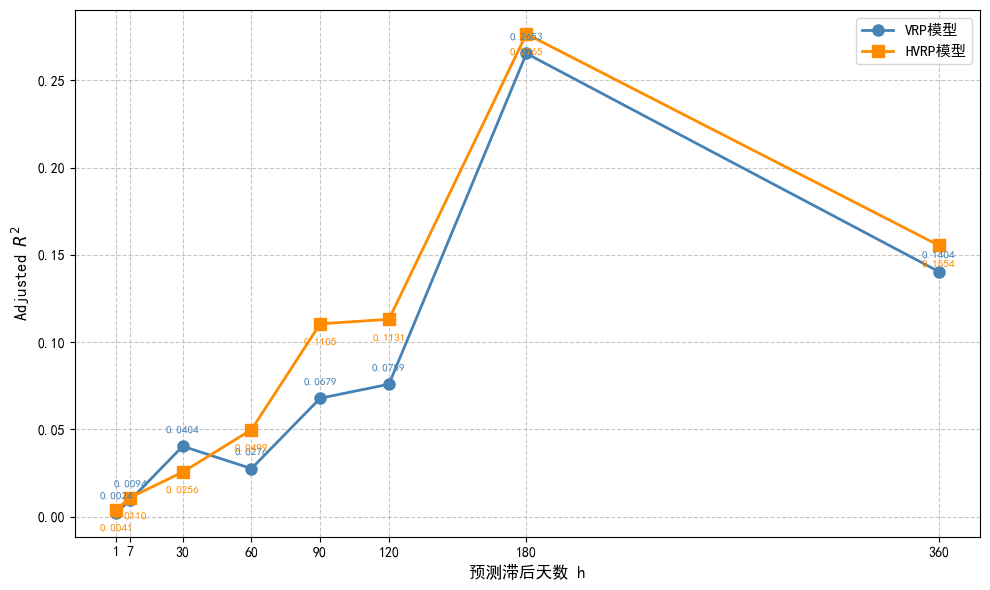
\includegraphics[width=\linewidth]{r2.png}
    \end{column}
    \begin{column}{0.42\linewidth}
      \begin{itemize}
        \item 60 日以上，HAR-VRP 多数窗口拟合度更高。
        \item 180 日窗口达到峰值。
        \item 但样本内 $R^2$ 不能单独证明预测优越性。
      \end{itemize}
    \end{column}
  \end{columns}
\end{frame}

\begin{frame}{审稿问题一：VRP 的经济定义要站稳}
  \begin{block}{当前风险}
    论文用 $VRP_t=IV_t-RV_t$，但经典文献中的 variance risk premium 通常是
    risk-neutral expected variance 与 physical expected variance 的差。
  \end{block}

  \begin{itemize}
    \item 若保持波动率单位，应称为 \textbf{volatility premium proxy}。
    \item 必须补充方差单位稳健性：$IV_t^2-\widehat{E}^{P}_t(RV)$。
    \item 30 日 MFIV 应与 30 日物理波动率期望匹配。
  \end{itemize}

  \[
    \widehat{RV}^{(30)}_{t}
    = \frac{1}{30}\sum_{j=1}^{30}\widehat{RV}_{t+j|t}
  \]
\end{frame}

\begin{frame}{审稿问题二：HAR-VRP 必须是实时可行预测}
  \begin{block}{审稿人会问}
    HAR-RV 是用全样本估计后生成 fitted value，还是用 rolling/expanding window 做实时预测？
  \end{block}

  \begin{itemize}
    \item 如果用全样本 HAR 系数，早期样本的 HVRP 会含有未来信息。
    \item 正确写法：每个 $t$ 只使用 $t$ 日以前信息估计 HAR，并生成 $\widehat{RV}_{t+j|t}$。
    \item ``HAR-VRP outperforms'' 必须基于样本外检验，而不是样本内调整 $R^2$。
  \end{itemize}

  \begin{exampleblock}{可替换句}
    For each forecast origin $t$, the HAR-RV coefficients are estimated recursively using information available up to $t$ only.
  \end{exampleblock}
\end{frame}

\begin{frame}{审稿问题三：长期预测回归的推断要更严}
  \begin{itemize}
    \item 因变量是 $h$ 日累计收益，$h=180$ 和 $360$ 时重叠非常严重。
    \item Newey-West lag $h-1$ 是必要条件，但通常不够。
    \item VRP 等预测变量具有持久性，长期预测 t 值容易偏乐观。
  \end{itemize}

  \vspace{0.25cm}
  \begin{block}{建议补充}
    非重叠月度/季度抽样、moving-block bootstrap、fixed-b 标准误、多重检验调整。
  \end{block}
\end{frame}

\begin{frame}{模型比较部分应成为修改重点}
  \begin{columns}[T,totalwidth=\linewidth]
    \begin{column}{0.48\linewidth}
      \begin{block}{当前已有}
        \begin{itemize}
          \item PDF 中出现 MSE
          \item 出现 $R^2_{OOS}$
          \item 出现 DM 与 MCS
        \end{itemize}
      \end{block}
    \end{column}
    \begin{column}{0.48\linewidth}
      \begin{alertblock}{当前不足}
        \begin{itemize}
          \item 模型 1--4 的含义不清
          \item benchmark 没有说明
          \item DM 正负方向和 p 值解释不清
          \item 嵌套模型应补 Clark-West
        \end{itemize}
      \end{alertblock}
    \end{column}
  \end{columns}

  \vspace{0.25cm}
  建议把第 6 节改成全文关键证据，而不是附带稳健性。
\end{frame}

\begin{frame}{建议新增的核心实验}
  \small
  \begin{tabularx}{\linewidth}{@{}p{0.18\linewidth}Y Y@{}}
    \toprule
    优先级 & 实验 & 解决的问题 \\
    \midrule
    必做 & 30 日期限匹配 VRP & 修复 IV 与 RV 期限错配 \\
    必做 & 递归 HAR-VRP & 排除未来信息泄露 \\
    必做 & 样本外 $R^2_{OOS}$ & 支撑 ``HAR 优于 VRP'' \\
    必做 & Clark-West / DM / MCS & 给模型优劣正式统计证据 \\
    必做 & 非重叠与 bootstrap & 修复长期重叠收益推断 \\
    强烈建议 & 方差单位 VRP & 对齐经典 variance risk premium 文献 \\
    强烈建议 & 状态依赖回归 & 支撑风险补偿 vs 情绪修正机制 \\
    \bottomrule
  \end{tabularx}
\end{frame}

\begin{frame}{文字层面的具体修改}
  \begin{enumerate}
    \item 标题突出期限结构反转，而不是泛泛地 ``pricing volatility risk''。
    \item 摘要中把 ``consistently outperforms'' 改为有条件表述，等样本外检验补齐后再强化。
    \item 引言少写市场背景，多写研究 puzzle、变量难点和预测时点。
    \item 方法部分新增 ``timing convention''：预测变量在 $t$ 日收盘可得，收益从 $t+1$ 到 $t+h$。
    \item 结论中把 ``reflects risk compensation'' 改为 ``is consistent with risk compensation''。
  \end{enumerate}
\end{frame}

\begin{frame}{建议后的论文主线}
  \begin{enumerate}
    \item \textbf{主问题}：CSI 300 ETF 期权中的 VRP 是否预测未来收益？
    \item \textbf{主事实}：预测符号存在期限结构反转。
    \item \textbf{分解}：上行与下行 semivariance premium 的信息衰减不同。
    \item \textbf{方法}：HAR-RV 过滤物理波动率噪声。
    \item \textbf{验证}：递归样本外预测、DM/Clark-West、MCS。
    \item \textbf{解释}：风险补偿与情绪修正并存，但需要状态依赖检验支撑。
  \end{enumerate}
\end{frame}

\begin{frame}{最终修改路线图}
  \begin{block}{第一轮：先修可信度}
    明确 VRP 单位、期限匹配、预测时点、HAR 递归估计。
  \end{block}

  \begin{block}{第二轮：再修证据链}
    补充样本外预测、非重叠/Bootstrap 推断、方差单位稳健性。
  \end{block}

  \begin{block}{第三轮：最后修叙事}
    把全文主线改为 ``期限结构反转 + 不对称信息 + HAR 过滤是否带来预测增益''。
  \end{block}
\end{frame}

\begin{frame}{一句话总结}
  \Large
  这篇论文有一个值得保留的核心发现：

  \vspace{0.4cm}
  \begin{center}
    \textbf{中国 CSI 300 ETF 期权市场中的 VRP 预测信息不是单调的，\\
    而是具有明显的期限结构反转与上下行不对称。}
  \end{center}

  \vspace{0.4cm}
  \normalsize
  但要让这个发现达到可发表标准，必须补齐四个环节：
  \textbf{定义、期限、实时预测、样本外比较}。
\end{frame}

\end{document}

